\begin{frame}
  \frametitle{Reducing the gEPK with SVD}

Take a model, $f(x, \theta)$, which satisfies the necessary conditions for expression as:
 \begin{align}
     f(x, \theta_\text{tr}) &= f(x, \theta_0(0)) +  \sum_s
\int_0^1                                  \left\langle 
                                   \varphi_{s,t}(x) , \sum_i
                                   \left(\dfrac{dL(x_i, y_i)}{df(x_i,
                                   \theta_s(0))} \varphi_{s,
                                   0}(x_i)\right) \right \rangle dt\\
     \varphi_{s,t}(x) &= \nabla_\theta f(x, \theta_s(t))
 \end{align}
Then we will let the RHS be rows of a matrix $L \cdot A$ where $L =
$diag($\dfrac{dL(x_i, y_i)}{df(x_i, \theta_s(0))})$ and each row $A_i
= \varphi_{s,0}(x_i)$. Then we can compute $U\Sigma V^T =
A$. We will truncate $V$ and rewrite
\begin{align}
     f(x, \theta_\text{tr}) &= f(x, \theta_0(0)) +  \sum_s
\int_0^1                                  \left\langle 
                                   \varphi_{s,t}(x) , \sum_k
                                   a_k\sigma_k V_k \right \rangle dt\\
\end{align}
Where $a_k$ is computed from the loss gradients and $\sigma_k$ is the
$k^{\text{th}}$ singular value.
% into $V'$ and now use $V'^T$ as our reference tangent space. Then we
% can project $L$ onto the same basis and rewrite $L \cdot A$ as
% \begin{align}
%   V' L U^T U A V'^T
% \end{align}

\end{frame}

\section{Conclusions and Outlook}
\label{Chapter5} % Change X to a consecutive number; for referencing this chapter 
\begin{frame}
  \frametitle{Conclusion : Next Direct Results}
  \begin{itemize}
    \item In addition to making the above replacement with SVD, random
      features may be a cheap alternative with similar performance.
    \item A more general spectral form is possible, using features
      which span multiple training steps. Random Fourier Features may
      be a nice cheap way to accomplish this.
    \item Decomposition of (adversarial) input gradients according to
      the principal components from the training inputs (or principal
      components using the SVD formulation above).

\begin{align}
  f(x, \theta_F) &= f(x, \theta_0) + \sum_i \sum_s \int_0^1 \langle
  \nabla_\theta f(x, \theta_s(t)), f(x_i, \theta_s(t))\rangle dt \\
  \dfrac{d f(x, \theta_F)}{dx} &= \dfrac{d f(x, \theta_0)}{dx} + \sum_i \sum_s \int_0^1 \langle
  \nabla_\theta \dfrac{d f(x, \theta_s(t))}{dx}, f(x_i,
                                 \theta_s(t))\rangle dt.
\end{align}
  \end{itemize}    
\end{frame}
\begin{frame}
  \frametitle{Conclusion : Next Applications}
\begin{figure}[ht!]
    \centering
    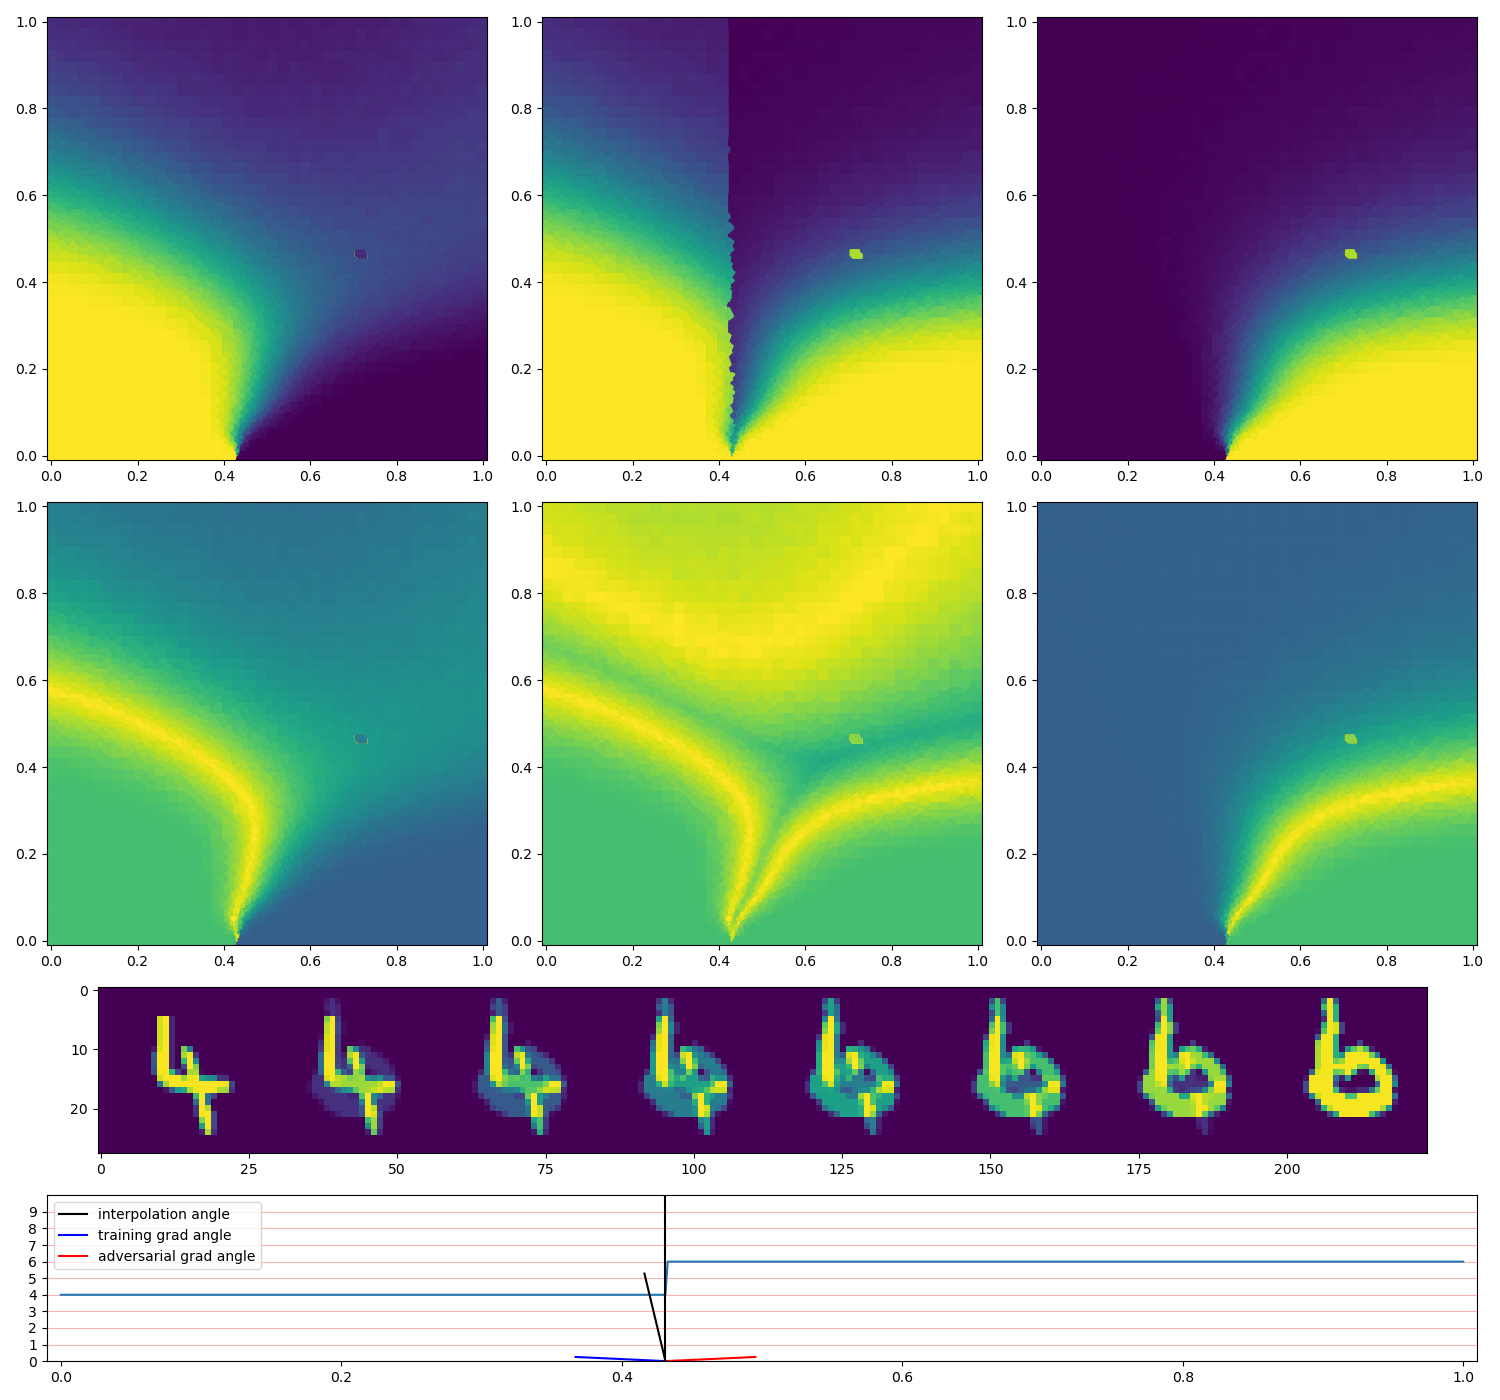
\includegraphics[width=0.42\textwidth]{c5_figures/stab-mnist-C32-50-50-10-0.001-eval-1e-06-none-4-6-db_interp-stability-50.png}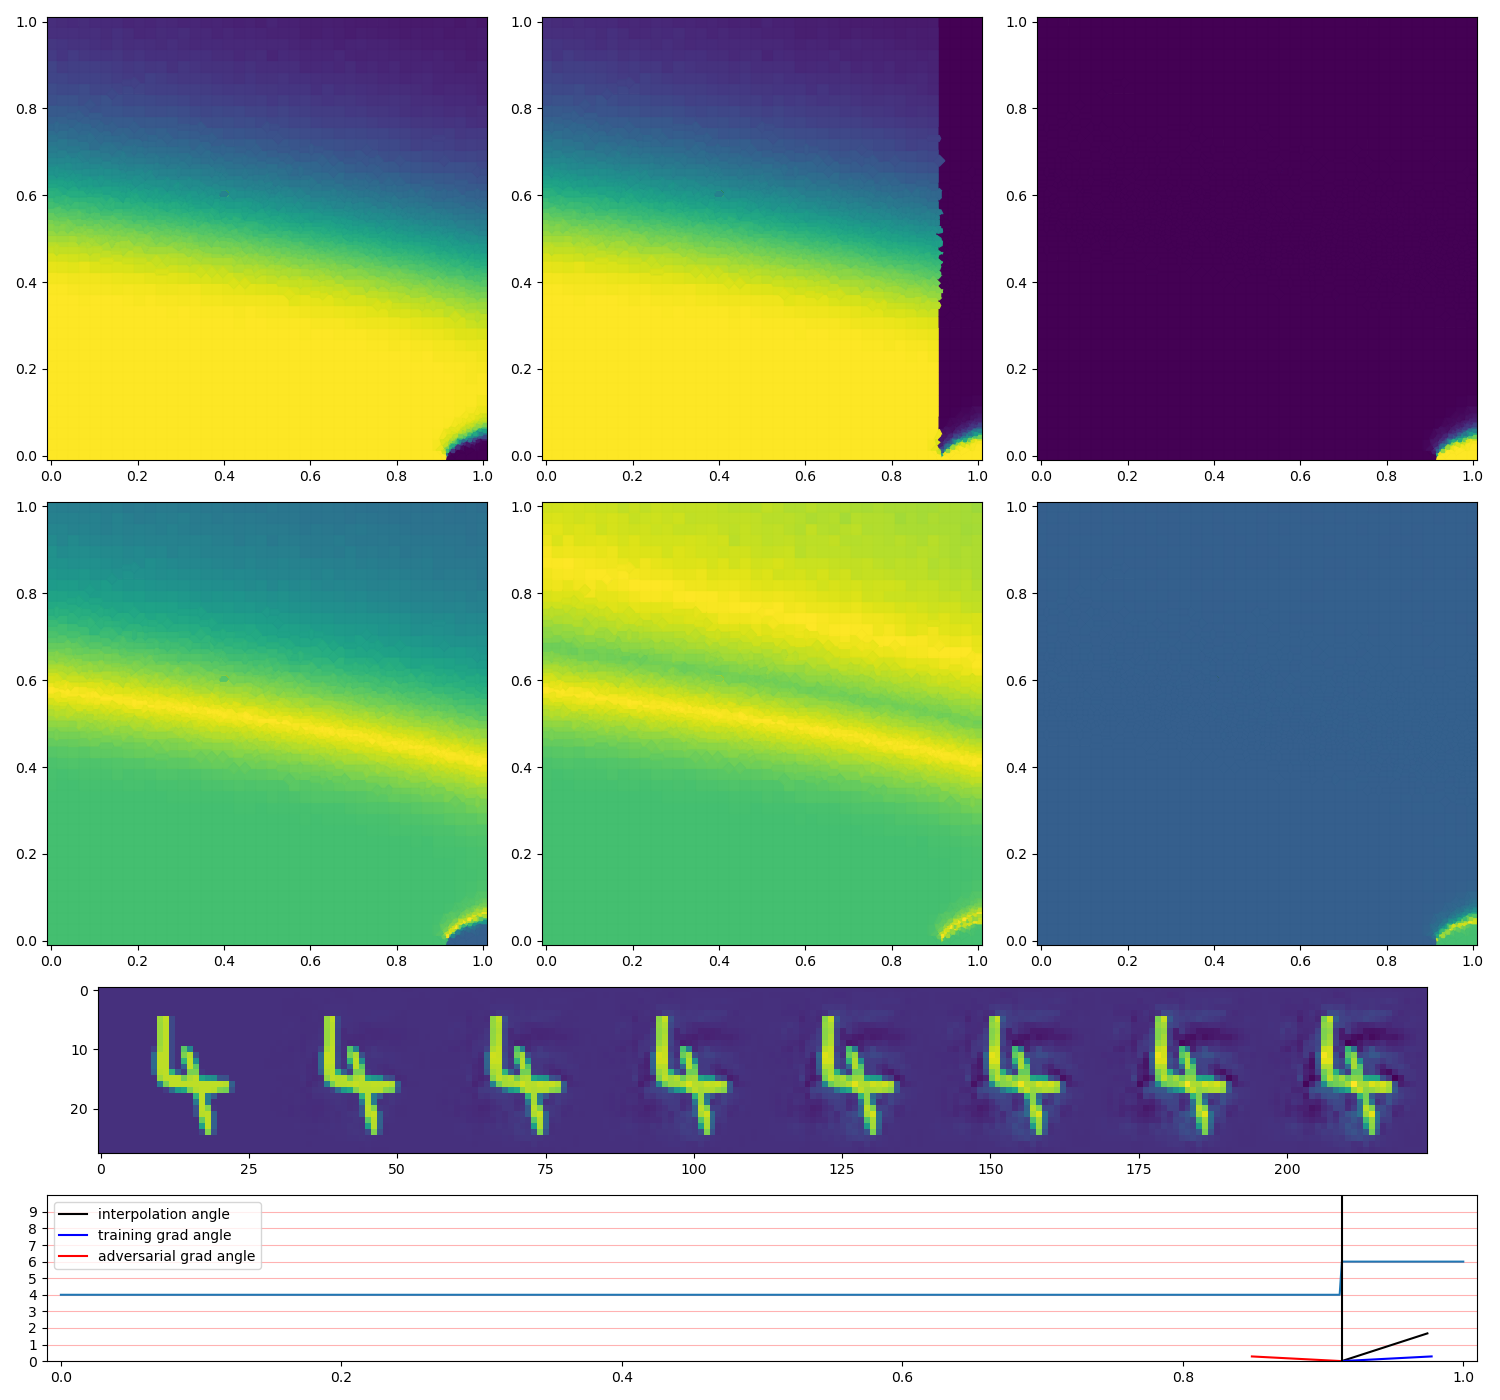
\includegraphics[width=0.42\textwidth]{c5_figures/stab-mnist-C32-50-50-10-0.001-eval-1e-06-pgd-4-6-db_interp-stability-50.png}
%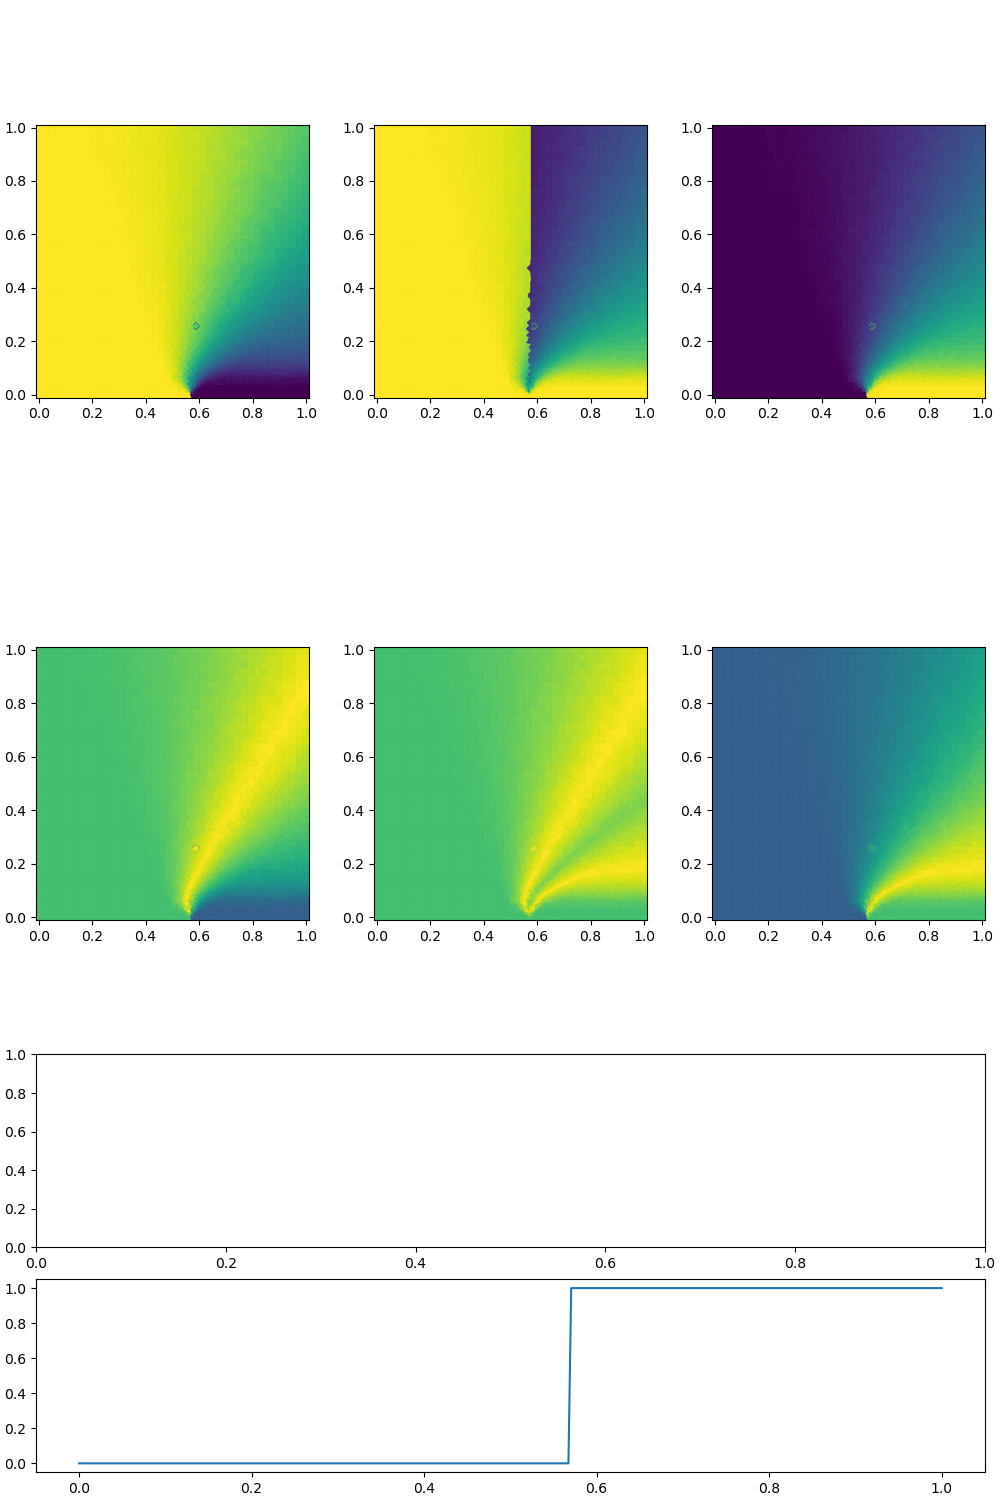
\includegraphics[width=0.9\textwidth]{c5_figures/wedge-mnist-C32-50-50-10-0.001-eval-1e-06-pgd-1-7-db_interp-stability-0.png}

    % 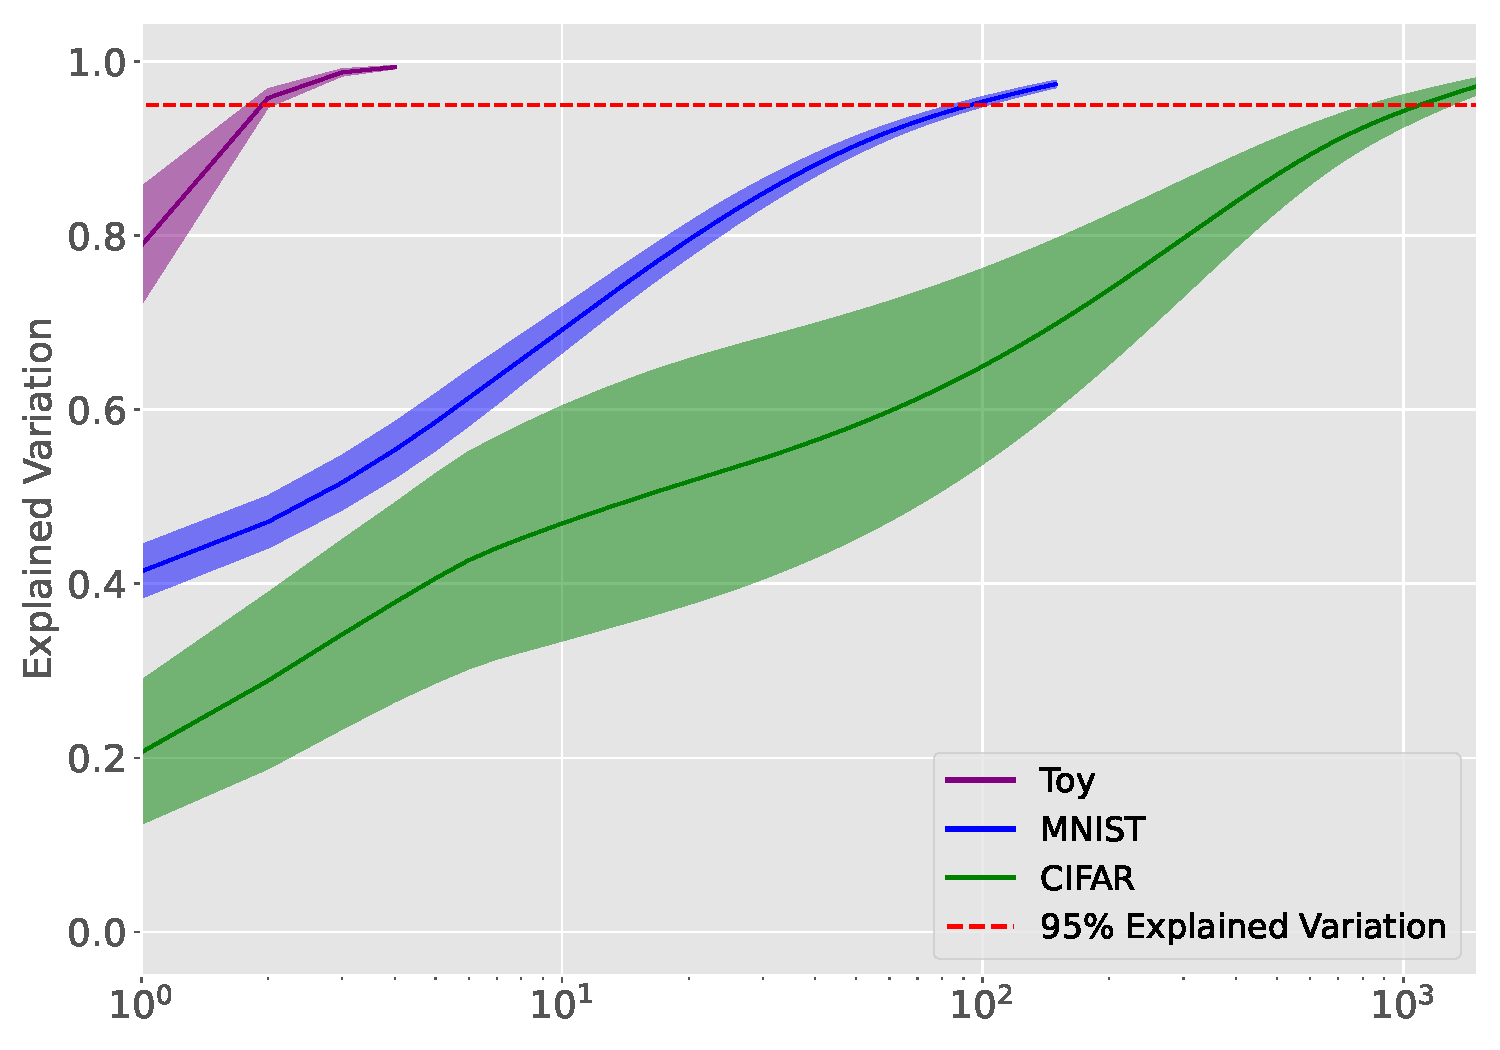
\includegraphics[width=0.45\textwidth]{c4a_figures/dimensionality_means.pdf}
\end{figure}

Decision boundary curvature can now be analyzed directly using
decompositions based on the gEPK. 
\end{frame}

\begin{frame}
  \frametitle{Conclusion}
  Today, you have heard about
  \begin{itemize}
  \item Geometric observations about adversarial attacks using a novel
    soft spatial metric (Submitted to CoDA 2023).
  \item A brand new method for representing neural networks in terms
    of blinear maps which admits useful decompositions and provides a
    robust theoretical framework for analysis. (Accepted NeurIPS
    TAG-ML Proceedings)
    \item Analysis explaining cutting edge OOD detection using this
      kernel representation framework and showing that these
      techniques are in general subsets or reductions of the subspaces
      revealed by this representation. (Submitted to ICLR 2024)
      \item Connections between geometric properties and robustness
        which can be explored by applying these techniques. 
\end{itemize}
\end{frame}
% \begin{frame}
%   \frametitle{Further Future Work}

%   \begin{itemize}
%   \item Due to the asymmetry observed in this kernel method, these
%     functionals cannot be limited to Hilbert space.
%     \item Derive a Banach space with reproducing kernels in which
%       these functionals can be embedded.
%       \item Leverage the properties of this banach space to apply
%         convergence and accuracy bounds. 

%   \end{itemize}
% \end{frame}




% elsewhere, use \ref{Chapter5}

% Throughout this work, I have sought to understand the intrinsic
% structure of machine-learning models and how this gives
% rise to adversarial attacks. I began by studying the construction of
% neural networks in Chapter. ~\ref{Chapter1} and learning in practice by generating adversarial
% attacks in Chapter. ~\ref{Chapter2}. This led naturally to a more careful study of decision
% boundaries and the development of the Persistence metric in Chapter
% 3. ~\ref{Chapter3}. Uncanny drops in persistence while crossing
% decision boundaries toward adversarial attacks indicated that attacks
% may exist in highly curved regions. The field conspicuously lacks
% tools for evaluating curvature, although some progress is being
% made. In the process of lit review for methods that would allow more
% direct analysis I discovered deficiencies in nascent literature on
% path kernels starting with the work of ~\citet{domingos2020}. The
% initial work to correct these deficiencies and produce an exact path
% kernel are presented in Chapter ~\ref{Chapter4}. This new exact path kernel
% representation for neural networks has a primary advantage which is to
% decompose model predictions into contributions from each training
% point. This decomposition is in the form of decomposing a prediction
% in a tangent space, where the exact path kernel implicitly maps the
% training data into a given tangent space. This mapping can be done for
% parameter gradients, input space gradients, and several dual tangent
% spaces related to both of these. Two such decompositions are applied
% in Chapter. ~\ref{Chapter4a} to demonstrate that many cutting edge OOD
% detection algorithms implicitly use this decomposition in terms of
% parameter gradients, and that the dual of the input gradients can be
% used to measure signal manifold dimension.

% We can summarize the first 3 chapters as posing some fundamental
% geometric questions related to machine-learning robustness. 
% Chapters 4 and 5 as propose a new framework for analyzing geometric
% properties and demonstrating that this framework can be applied very
% generally. From here, there are several important directions for
% future research. First is the application of these methods directly to
% the adversarial robustness questions from Chapters 1-3. Second is the
% complete generalization of this new framework including conditions
% under which such representations live in Banach spaces or Hilbert
% spaces and what order of accuracy can be maintained using truncated
% spectral decompositions. Third is the application of this theory more
% broadly to the wide variety of spatial problems that are present in
% machine-learning. 

% \subsection{Applications to Adversarial Robustness}



% In Fig. ~\ref{fig:dbs} we can see that sharp geometric curvature
% and shallow angles are observed when interpolating across decision
% boundaries between natural and especially adversarial images. One line
% of research will follow the direct geometric approach by constructing
% test objects (wedges) which replicate the structure observed in the
% practical networks. an example of this is shown in ~\ref{fig:dbs}. The
% second approach is to take advantage of the framework from Chapters
% ~\ref{Chapter4} and ~\ref{Chapter4a} in order to decompose the
% training gradients at points on the decision boundary to understand
% neural networks' learned degrees of freedom at these locations. The
% goal of this line of research is to understand these geometric
% constraints and eventually pose both updated training objectives and
% also better definitions for the identification of adversarial examples
% in practice. This line of research may have implications beyond
% robustness, to include uncertainty quantification, generalization,
% out-of-distribution detection, and other useful metrics to create
% ptrustworthy AI.

% From this decomposition, we can also replace the individual training
% data with an orthogonal basis by choosing vectors as in
% ~\citet{halko2011finding}, solving SVD for each step, or more
% generally, we can define spectral components across all training steps
% and perform more general spectral decomposition with further
% efficiency reduction as in ~\citet{tancik2020fourierfeatures}. The path kernel
% formulation allows easy management of numerical error for any of these
% approaches. 

% Regardless of how sophisticated we make this decomposition, all of
% these methods have the advantage of maintaining an exact mapping to
% the tangent space around each input point. This mapping implicitly
% defines natural dimension reduction -- by truncating the chosen
% basis. The tangent space can be thought of as the models implicit
% justifications -- which training influences are affecting its
% decisions on this prediction. These directions are implicitly how we
% can analyze (and potentially penalize) points of high curvature
% e.g. at the decision boundary. This provides a theoretical foundation
% from which recent work in manifold study and data augmentation
% ~\citep{kaufman_data_2023, liu_linear_2023, sipka_differentiable_2023,
%   cha_orthogonality-enforced_2023, marbut_reliable_2023,
%   gao_out--domain_2023, oh_provable_2023, chen2023aware}.


% \subsection{Generalization in the sense of Reproducing Kernel Banach Spaces}
% Given that the representation from Chapters ~\ref{Chapter4} and
% ~\ref{Chapter4a} have a small asymmetry, a general description of
% these representations cannot fit within Hilbert Space. There is a
% convenient approach building on the theory of Reproducing Kernel
% Banach Spaces (RKBS) which is summarized nicely by
% ~\citet{zhang2009reproducing}. It is by careful construction of a
% semi-inner product that I believe our representation can be written in
% this way. This allows access to tools built for Banach spaces for
% analysis of both accuracy, risk minimization, and other useful
% results. A similar line of work is already being pursued by
% ~\citet{shilton_gradient_2023} with which our work can likely be
% connected. I believe this is the most interesting natural direction
% for continuing work. Although this is less likely to produce practical
% payoffs immediately, I believe that this approach will greatly enhance
% the theoretical foundation upon which analysis of neural network
% performance and limitations are based. 

% \subsection{Connecting Distributional Learning with Neural Networks}

% The neural representations and decompositions proposed in this work
% provide images of the tangent space according to the
% a given model for each point in the data space. The tangent space
% for each datum must be connected within the implicit metric space of
% the neural network, helping us to pose constraints on the geodesics
% connecting data. It has been shown increasingly in recent work
% (e.g. by  ~\citet{lu2020universal}, ~\citet{yang2022capacity}, \citet{altekruger_neural_2023}) that Neural Networks
% learn distributions in a sense that approximates the Wasserstein
% metric to some order. Also, work by ~\citet{chizat2020maxmargin} that neural network
% classifiers are approximately max-margin classifiers in some
% implicit space. We cannot necessarily compute this space exactly,
% however by examining the tangent spaces exposed by the kernel type
% decomposition, we can pose questions about this metric space in the
% dual sense. The connection of these three concepts into an
% understanding of how Neural Networks embed an approximation of the
% Wasserstein metric into some implicit spaces that is likely
% euclidean will have significant impact on the machine-learning
% community at large. This method also serves to connect the prior
% work from Chapters 1-3 with this later work, examining how models
% connect data geometrically. 




